\chapter{Introduction}

This work has been carried out in cooperation with two academic institutions, University of Antwerp (UA) and Universidad Aut\'onoma de Madrid (UAM).

\section{Problem Description}

The context of this Master's Thesis is Domain Specific Modeling applied to Android development for the generation of collaborative applications. Domain-Specific Modeling (DSM) and Model Transformation (MT) have the potential to support rapid development and synthesis of new applications on Android. This thesis investigates the power and limitations of DSM and MT in the context of Android. The metaDepth meta-modeling framework and tool will be used to create a domain specific language (DSL) that allows the creation of collaborative Android applications.
\\ \\
This work arises from the rising need for mobile applications that solve recurring collaborative problems. The thesis tries to tackle those recurring problems by applying DSM on the Android stack to support collaborative work.

Leek wil ook Android apps maken. Specifiek voor zijn noden. Makkelijker met een DSL. Geen Java/Android SDK kennis vereist.

\section{Background}

In general, traditional software development follows a process that aims at guaranteeing a certain standard. Important stages in this process are \textit{specification}, \textit{implementation} and \textit{verification}. Software testing is an important aspect of this latter activity. Although the analysis of different software development processes is out of the scope of this thesis, it is an important contribution to the quality of a solution that solves a problem through DSM. In the following, these three stages are described as a natural evolution to DSM. Also \textit{code generation} is discussed as a possible solution to recurring software engineering problems.

\subsection{Specification}

Specification identifies the problems a new software system is suppose to solve, its operational capabilities, its desired performance characteristics, and the resource infrastructure needed to support system operation and maintenance \cite{ProcessModels}. Based on the requirements specification, software engineers can build an architectural design. The final goal of any engineering activity is to create some kind of documentation. If the design truly represents a complete system design, a team of software engineers can proceed to build iterations of the product, dependent on the software lifecycle that is applied. (http://c2.com/cgi/wiki?WhatIsSoftwareDesign)

\subsection{Implementation}

After creating a requirements specification and any accompanying design documents, a software engineering team can proceed to the implementation stage. An implementation usually is a realization of the design documents created in an earlier step. The result of the implementation stage is a software component or system that conforms as close as possible to those design documents.

\subsection{Verification}

Verification is the process of determining that a system, or a module, meets its specification. The verification process always relies on the requirements specification, as this document defines the intended behavior of the system. We could also ask ourselves \textit{"Are we building the system right?"}. Verification is usually performed by (automated) testing of the system. The testing process can involve unit testing (testing a component in isolation), integration testing (components tested as a group), regression testing (uncover new errors in existing functionality after changes have been made to a system) and other ways of verifying that the system behaves as we expect it to.
\\ \\
A complete software development lifecycle is depicted in figure \ref{fig:lifecycle}. One of the goals of this thesis is to minimize or even eliminate the implementation and testing cycles. Using a DSL, an end-user can easily create and customize their own applications by specifying its functionality in a clear and non-verbose way. The requirements and design lifecycle remain the same, as we use these documents to generate code. The activity of generating code is explained in the next subsection.

\begin{figure}[htb]
\centering
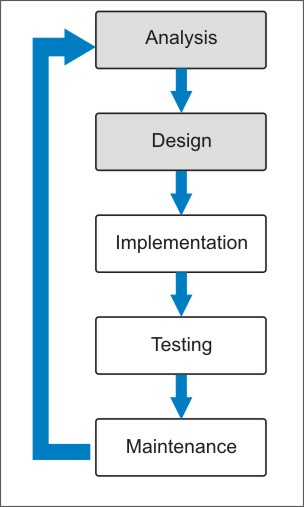
\includegraphics[width=0.6\textwidth]{images/lifecycle.jpg}
\caption{Software Development lifecycle}
\label{fig:lifecycle}
\end{figure}

\subsection{Code Generation}

When developing software, many bugs and errors occur due to coding mistakes in the implementation phase. This can happen due to reusing old software components, unimplemented methods, uninitialized variables, etc. In order to prevent those mistakes, we have to fall back onto coding standards in the development of software systems.
\\ \\
A possible approach is the use of code generation. Among the problems described earlier, it can also prevent errors that emerge in manually created code. Usually, a model (in e.g. UML) serves as a blueprint for generation the code. Sometimes the code generated from a UML diagram is not complete and merely offers stubs to the users that still have to be implemented manually. The main reason for this is that UML is a generic modeling language. However, if we constrain the required system to a restricted domain, we are able to generate specific code from a DSL. 

\section{Contribution}

\subsection{Aims and Objectives}

The goal of this Master's Thesis is to provide a coherent modeling framework for the creation of collaborative applications running on the Android platform. 
\\ \\
These are the main objectives of the study:

\begin{itemize}
\item{Discuss the shortcomings of two level modeling and why we need multi-level modeling}
\item{Analyze the possibilities of model driven engineering in the context of the Android platform}
\item{Analyze and define the different types of collaboration methods}
\item{Create a coherent framework that allows the creation of collaborative Android applications}
\end{itemize}

\subsection{Research Questions}

The research questions are sustained on underlying hypotheses. These are the main hypotheses with accompanying research questions:

\begin{itemize}
\item{Hypothesis 1. Android is an open source software stack. \\
Research Question 1. How can we leverage the Android stack to support the modeling of Android applications?}
\item{Hypothesis 2. There exists a categorization of different types of groupware options. \\
Research Question 2. How can we support the different types of groupware options in a modeling framework?}
\item{Hypothesis 3. The validation of the framework can be done based on certain quality attributes (QAs). \\
Research Question 3. Which QAs are needed to evaluate the framework properly?}
\end{itemize}

\subsection{Expected Outcomes}

These are the expected outcomes for this thesis:

\begin{itemize}
\item{A study of the possibilities of modeling Android applications}
\item{A study of the possibilities of multi-level meta-modeling}
\item{An ontology of collaboration patterns}
\item{A standardization of collaborative patterns in a framework (the collaboration stack)}
\item{A complete description and design of a modeling framework for collaborative applications}
\end{itemize}

\section{Thesis Outline}

This document starts with an overview of the fundamentals of domain specific modeling in chapter 2. It also explains why there are shortcomings in the two-level modeling approach. Chapter 3 continues with a solution (multi-level modeling) that resolves problems inherent to two-level modeling. It will also blabla Metadepth... Android dev... Collaborative shizzle... Case Study... Conclusion... Future Work!

